\begin{itemize}
    \item \add{Apresentação dos experimentos realizados: descrição dos cenários testados, procedimentos e configurações.}
    \item \add{Comparação dos resultados do SLAM\_toolbox com os dados do sistema OptiTrack, apresentando gráficos, mapas, trajetórias e análises quantitativas.}
    \item \add{Discussão dos resultados: análise dos pontos fortes e limitações da solução adotada, implicações para aplicações reais e comparação com os objetivos propostos.}
\end{itemize}

\section{Introdução}

\add{
\textbf{1. \txr{Objetivo do capitulo}}
Neste capítulo serão apresentados os resultados obtidos.....
\textbf{2. \txr{Temas a tratar}}
De tal modo, o capítulo inicia descrevendo o banco de dados utilizado para treinamento e teste das abordagens propostas, 
também são apresentados todos os resultados obtidos em diferentes etapas do processo, mostrando a evolução obtida a partir da implementação de algumas técnicas apresentadas anteriormente. 
E por fim, é feita uma análise destes resultados e uma comparação com os resultados obtidos por outros trabalhos semelhantes com o intuito de validar as abordagens propostas.
}


% ------------------ INICIO ----------------------
Utilizou-se a princípio a biblioteca SLAM Toolbox para criação de um mapa detalhado do laboratório, fazendo o robô percorrer diversos caminhos no interior do laboratório para que o mapa gerado fosse de alta qualidade e representativo do ambiente de testes. O mapa gerado por este método foi salvo e utilizado como mapa para os experimentos de localização do robô utilizando o modo de Localização da SLAM Toolbox (ver Figura \ref{fig:Exp_mapa_LABAIR}.

\begin{figure}[htb]
    \centering
    \caption{Mapa do LAB-AIR gerado com a SLAM Toolbox, mostrando os marcadores das posições e conexões do grafo de poses}
    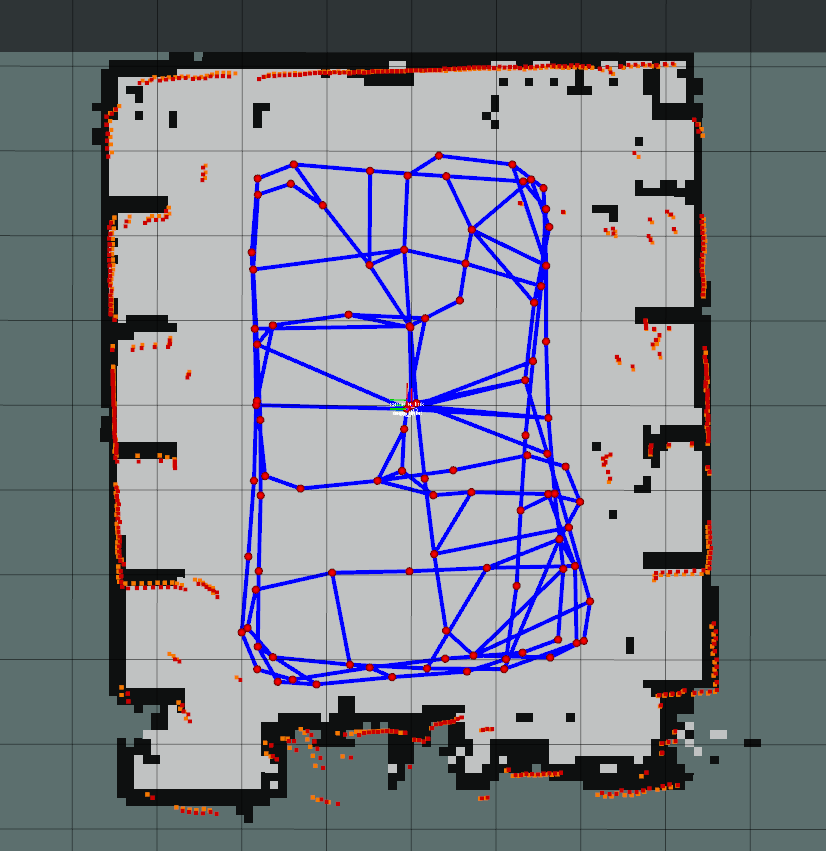
\includegraphics[width=0.5\linewidth]{img/mapa_localizacao.png}
    \source
    \label{fig:Exp_mapa_LABAIR}
\end{figure}

Para verificar o desempenho da tarefa de localização usando a SLAM Toolbox, utilizou-se o controlador definido na Seção \ref{sec:Controle_Dif_LIMO} para guiar o robô em dois tipos diferentes de trajetórias, uma caracterizada por caminhos lineares entre posições específicas no referencial inercial do laboratório, e uma trajetória em formato de Lemniscata de Bernoulli. As duas trajetórias podem ser vistas na Figura \ref{fig:exp_trajetorias}.

\begin{figure}
    \centering
    \caption{Trajetórias Realizadas nos Experimentos}
    \begin{subfigure}[b]{0.4\textwidth}
        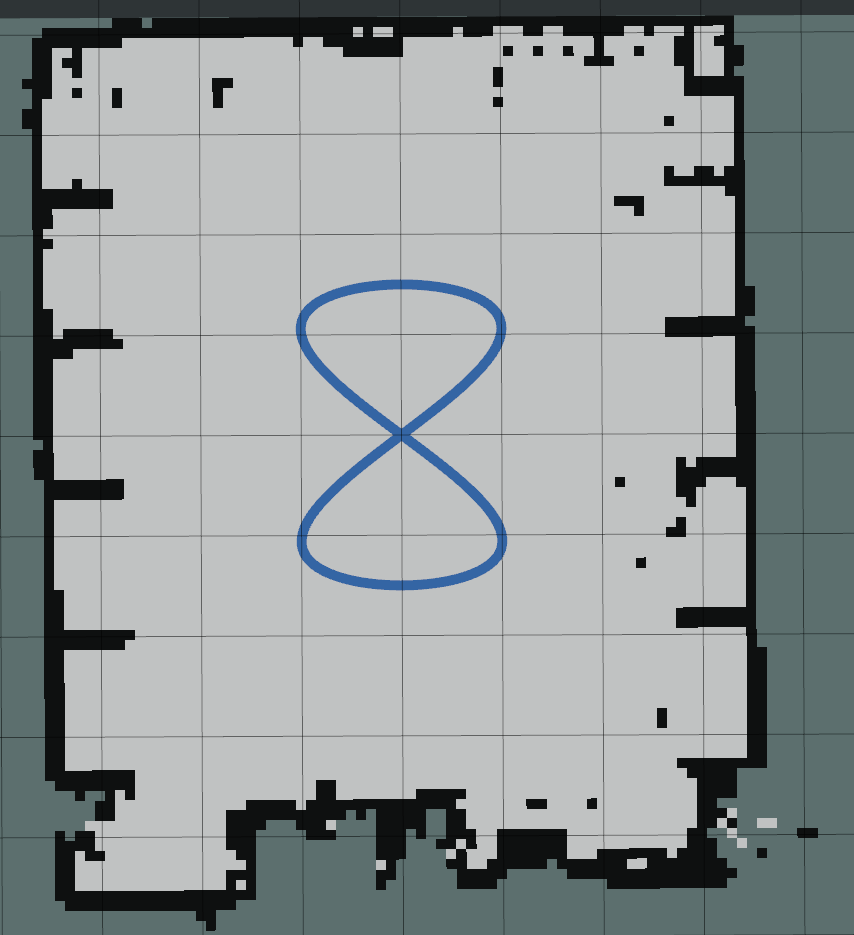
\includegraphics[width=\textwidth]{img/Trajetoria_Lemniscata.png}
        \caption{Trajetoria em Lemniscata de Bernoulli}
    \end{subfigure}
    \begin{subfigure}[b]{0.4\textwidth}
        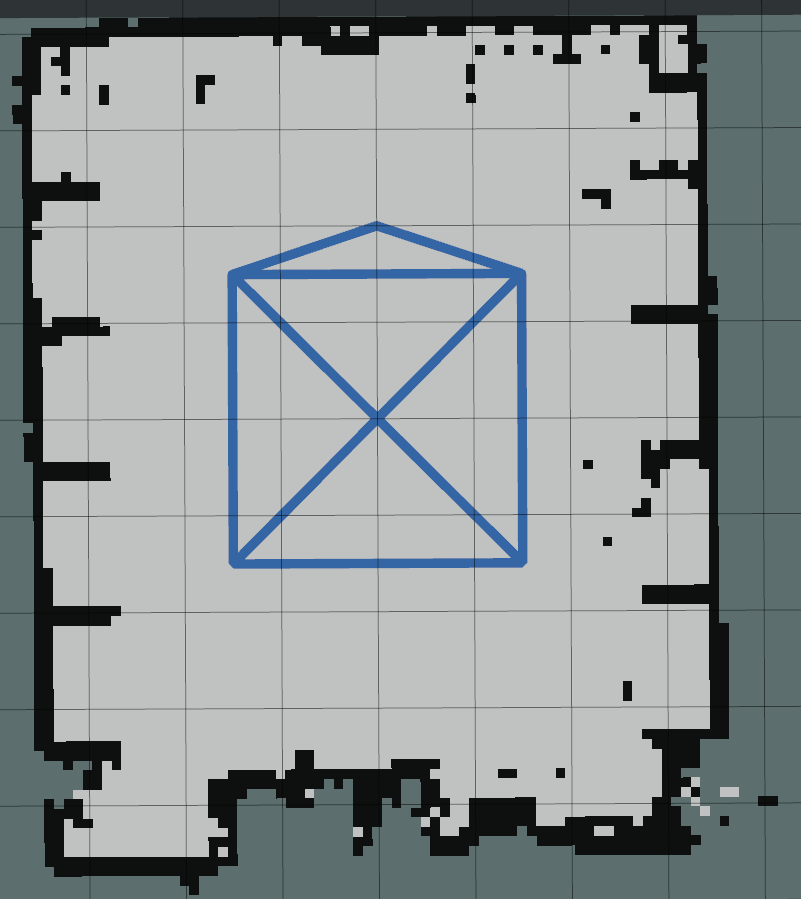
\includegraphics[width=\textwidth]{img/Trajetoria_Casa.png}
        \caption{Trajetória Linear}
    \end{subfigure}
    \label{fig:exp_trajetorias}
    \sourceParbox[0.8\linewidth]
\end{figure}

Para comparar o desempenho do sistema com o referencial do OptiTrack realizou-se 4 experimentos de controle de trajetória para cada uma das duas trajetórias definidas, usando primeiro informações provindas do sistema Optitrack para obter a pose do robô e posteriormente utilizando apenas as poses obtidas pela SLAM Toolbox.

Em todos os 4 experimentos armazenou-se tanto os dados de pose provindas do OptiTrack quanto da SLAM Toolbox, os sinais de controle calculados e enviados ao robô e a trajetória a ser seguida. A pose inicial do robô foi resetada ao início de cada experimento, mantendo o ponto $(0,0)$ do referencial inercial do laboratório como posição inicial e orientação paralela ao eixo $X$ ($\psi = 0 rad$).

O primeiro experimento realizado foi o controle de trajetórias lineares que formam uma figura de casa, ligando os pontos \add{inserir pontos}. A trajetória realizada e a trajetória desejada podem ser vistas na Figura \ref{fig:Trajetoria_VRPN_LINEAR}. Pode-se notar que a trajetória realizada pelo robô segue em grande parte a trajetória desejada, com alguns erros de seguimento da trajetória em pontos mais críticos de viradas mais bruscas e no início do experimento, quando o robô sai da origem do plano cartesiano e corre atrás do ponto da trajetória que está em movimento. A Figura \ref{fig:Exp1_Erros} mostra os erros de posição durante o experimento.

\begin{figure}[htb]
    \centering
    \caption{Trajetória realizada pelo robô no primeiro experimento}
    \begin{subfigure}[b]{0.49\textwidth}
         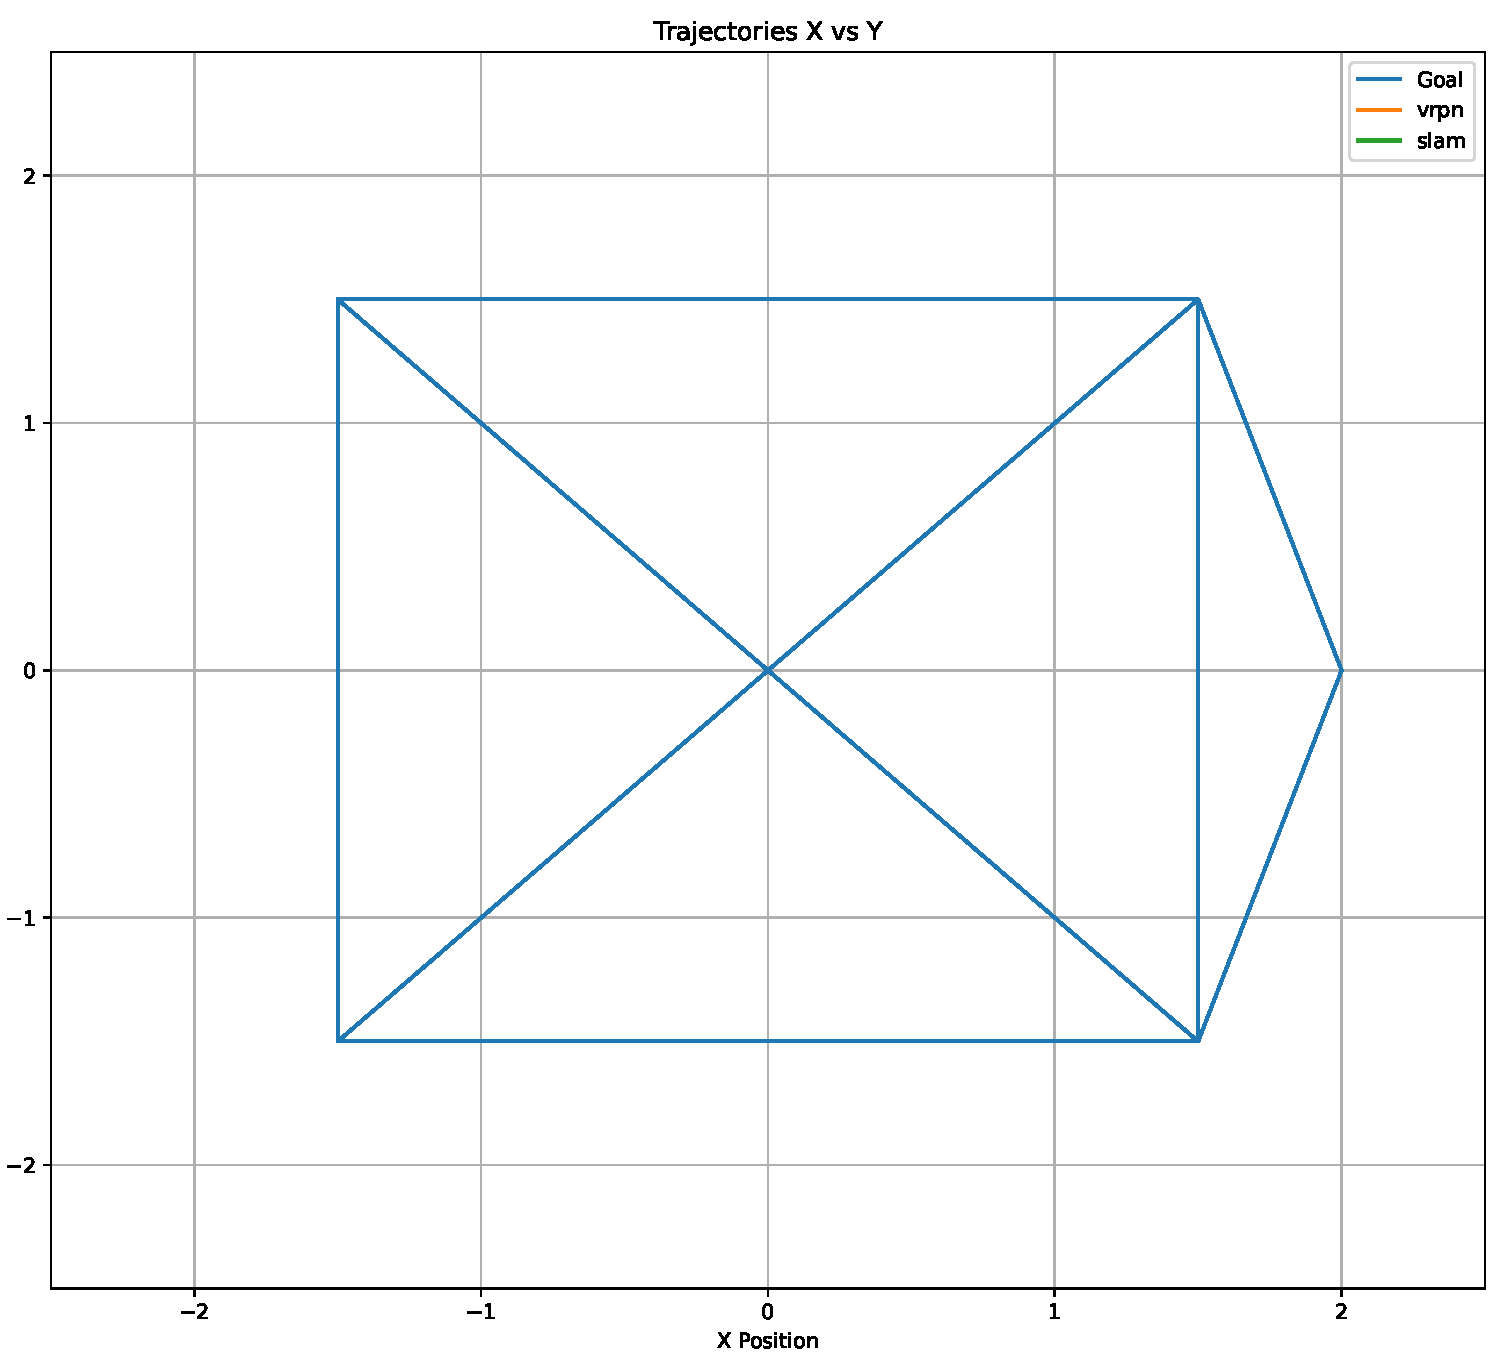
\includegraphics[width=\textwidth]{img/Resultados/Exp1_VRPN_Control_LINEAR/Trajetoria_Goal.pdf}
    \end{subfigure}
    \begin{subfigure}[b]{0.49\textwidth}
        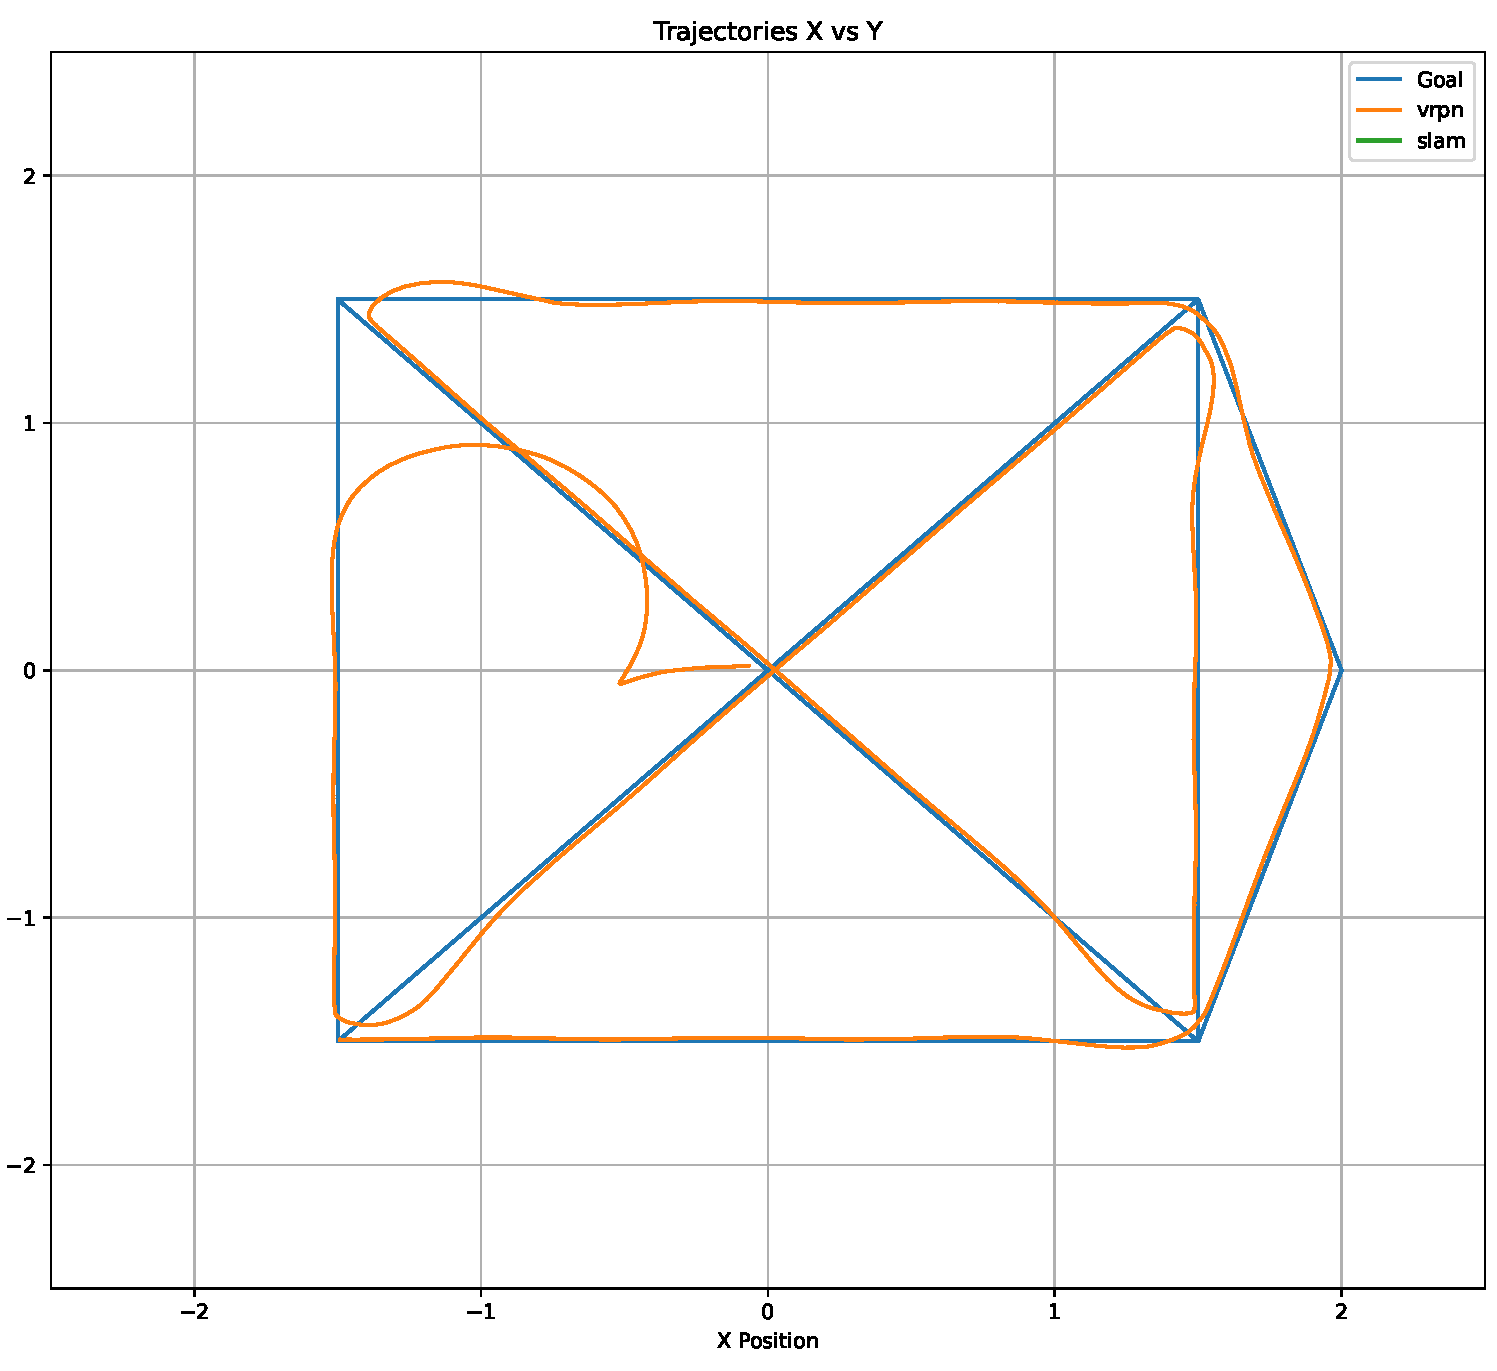
\includegraphics[width=\textwidth]{img/Resultados/Exp1_VRPN_Control_LINEAR/Trajetoria_VRPN_Goal.pdf}
    \end{subfigure}
    \source
    \label{fig:Trajetoria_VRPN_LINEAR}
\end{figure}

\begin{figure}[htb]
    \centering
    \caption{Trajetória Realizada + Pose obtida pela SLAM Toolbox}
    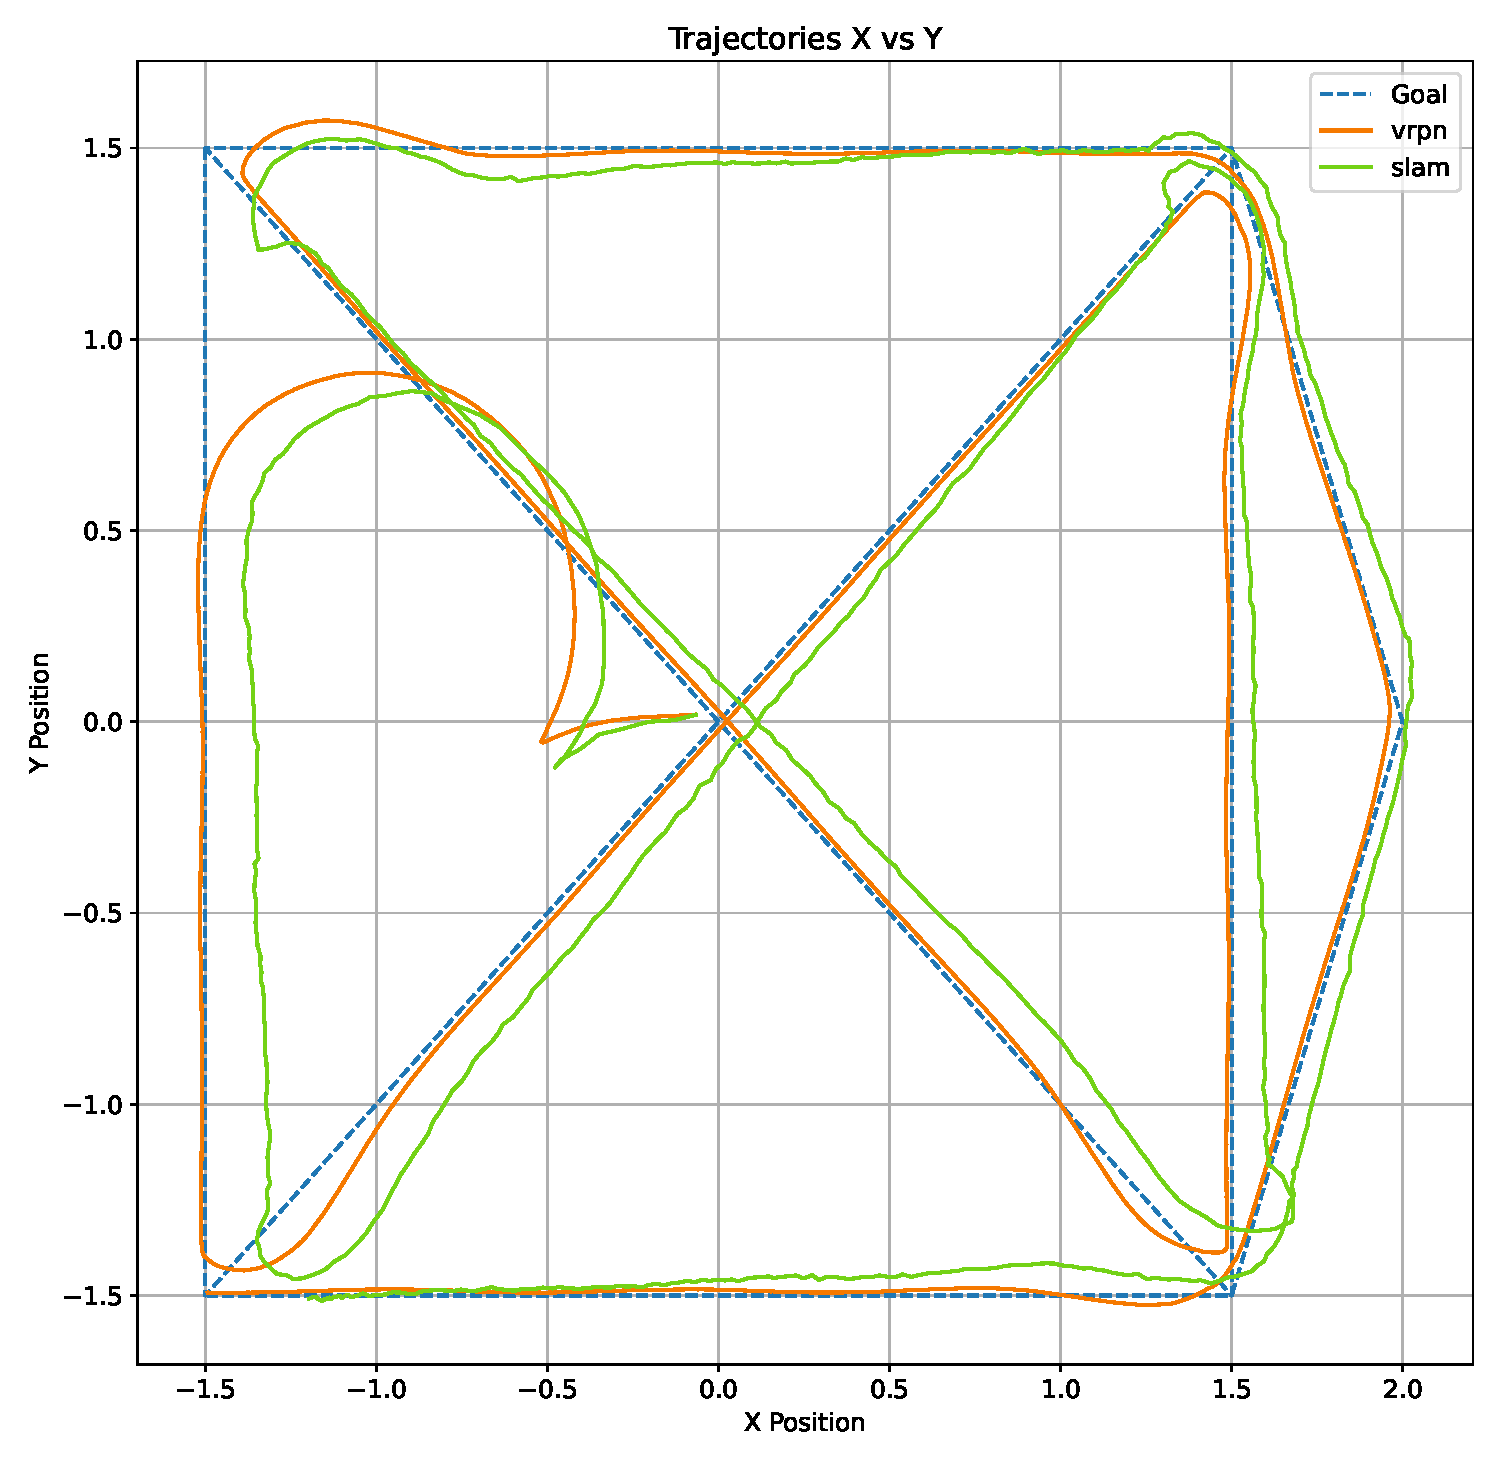
\includegraphics[width=0.8\linewidth]{img/Resultados/Exp1_VRPN_Control_LINEAR/Trajetoria_ALL.pdf}
    \label{fig:Exp1_Trajetoria_All}
\end{figure}

\begin{figure}[htb]
    \centering
    \caption{Evolução das coordenadas $x$ e $y$ no Experimento 1}
    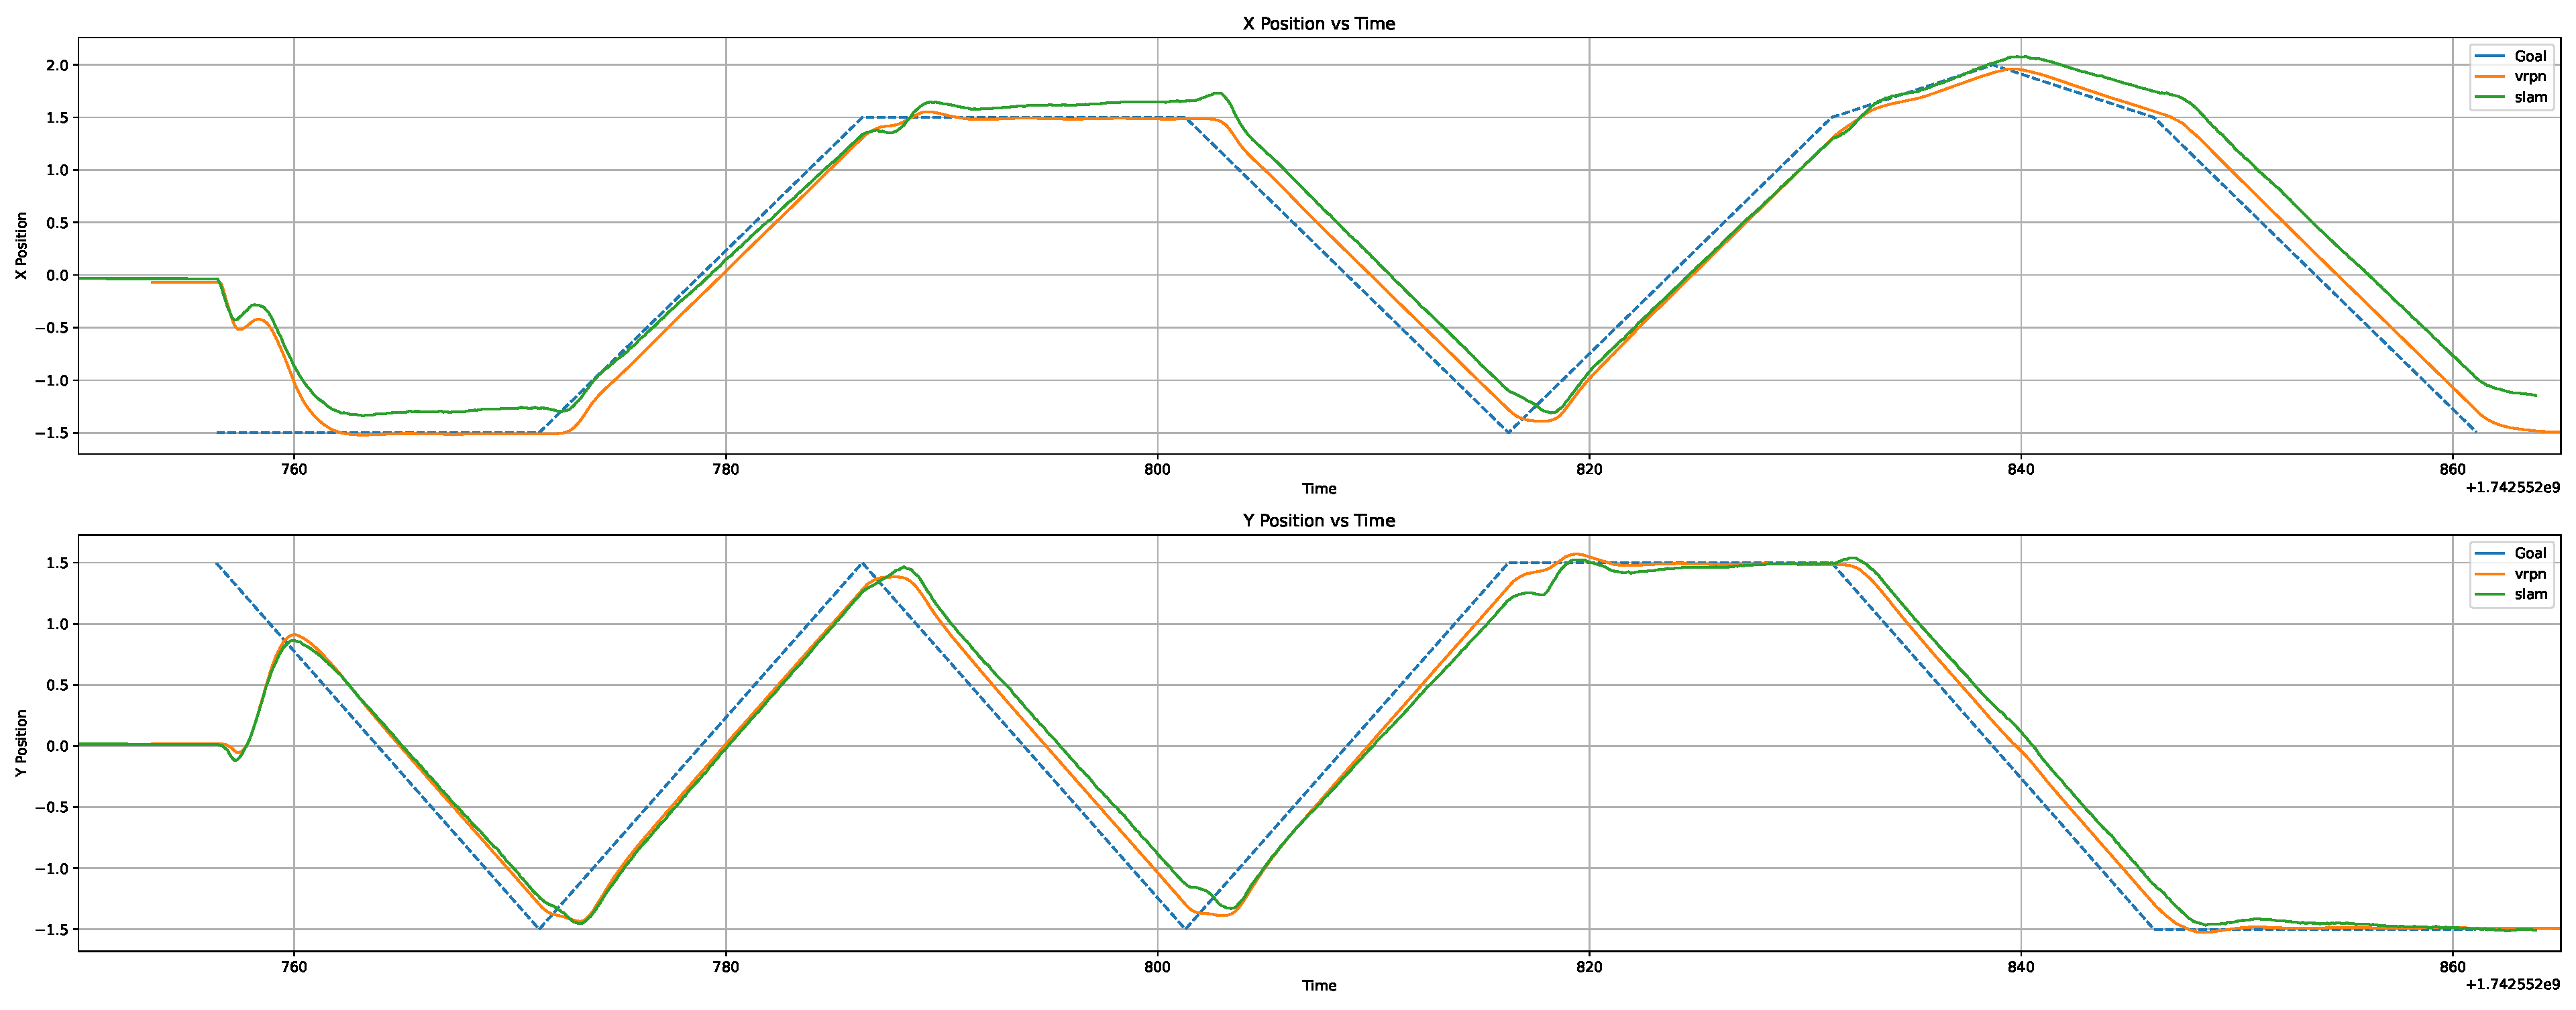
\includegraphics[width=\linewidth]{img/Resultados/Exp1_VRPN_Control_LINEAR/Position_v_time.pdf}
    \sourceParbox[\linewidth]
    \label{fig:Exp1_XY_vs_tempo}
\end{figure}

\begin{figure}
    \centering
    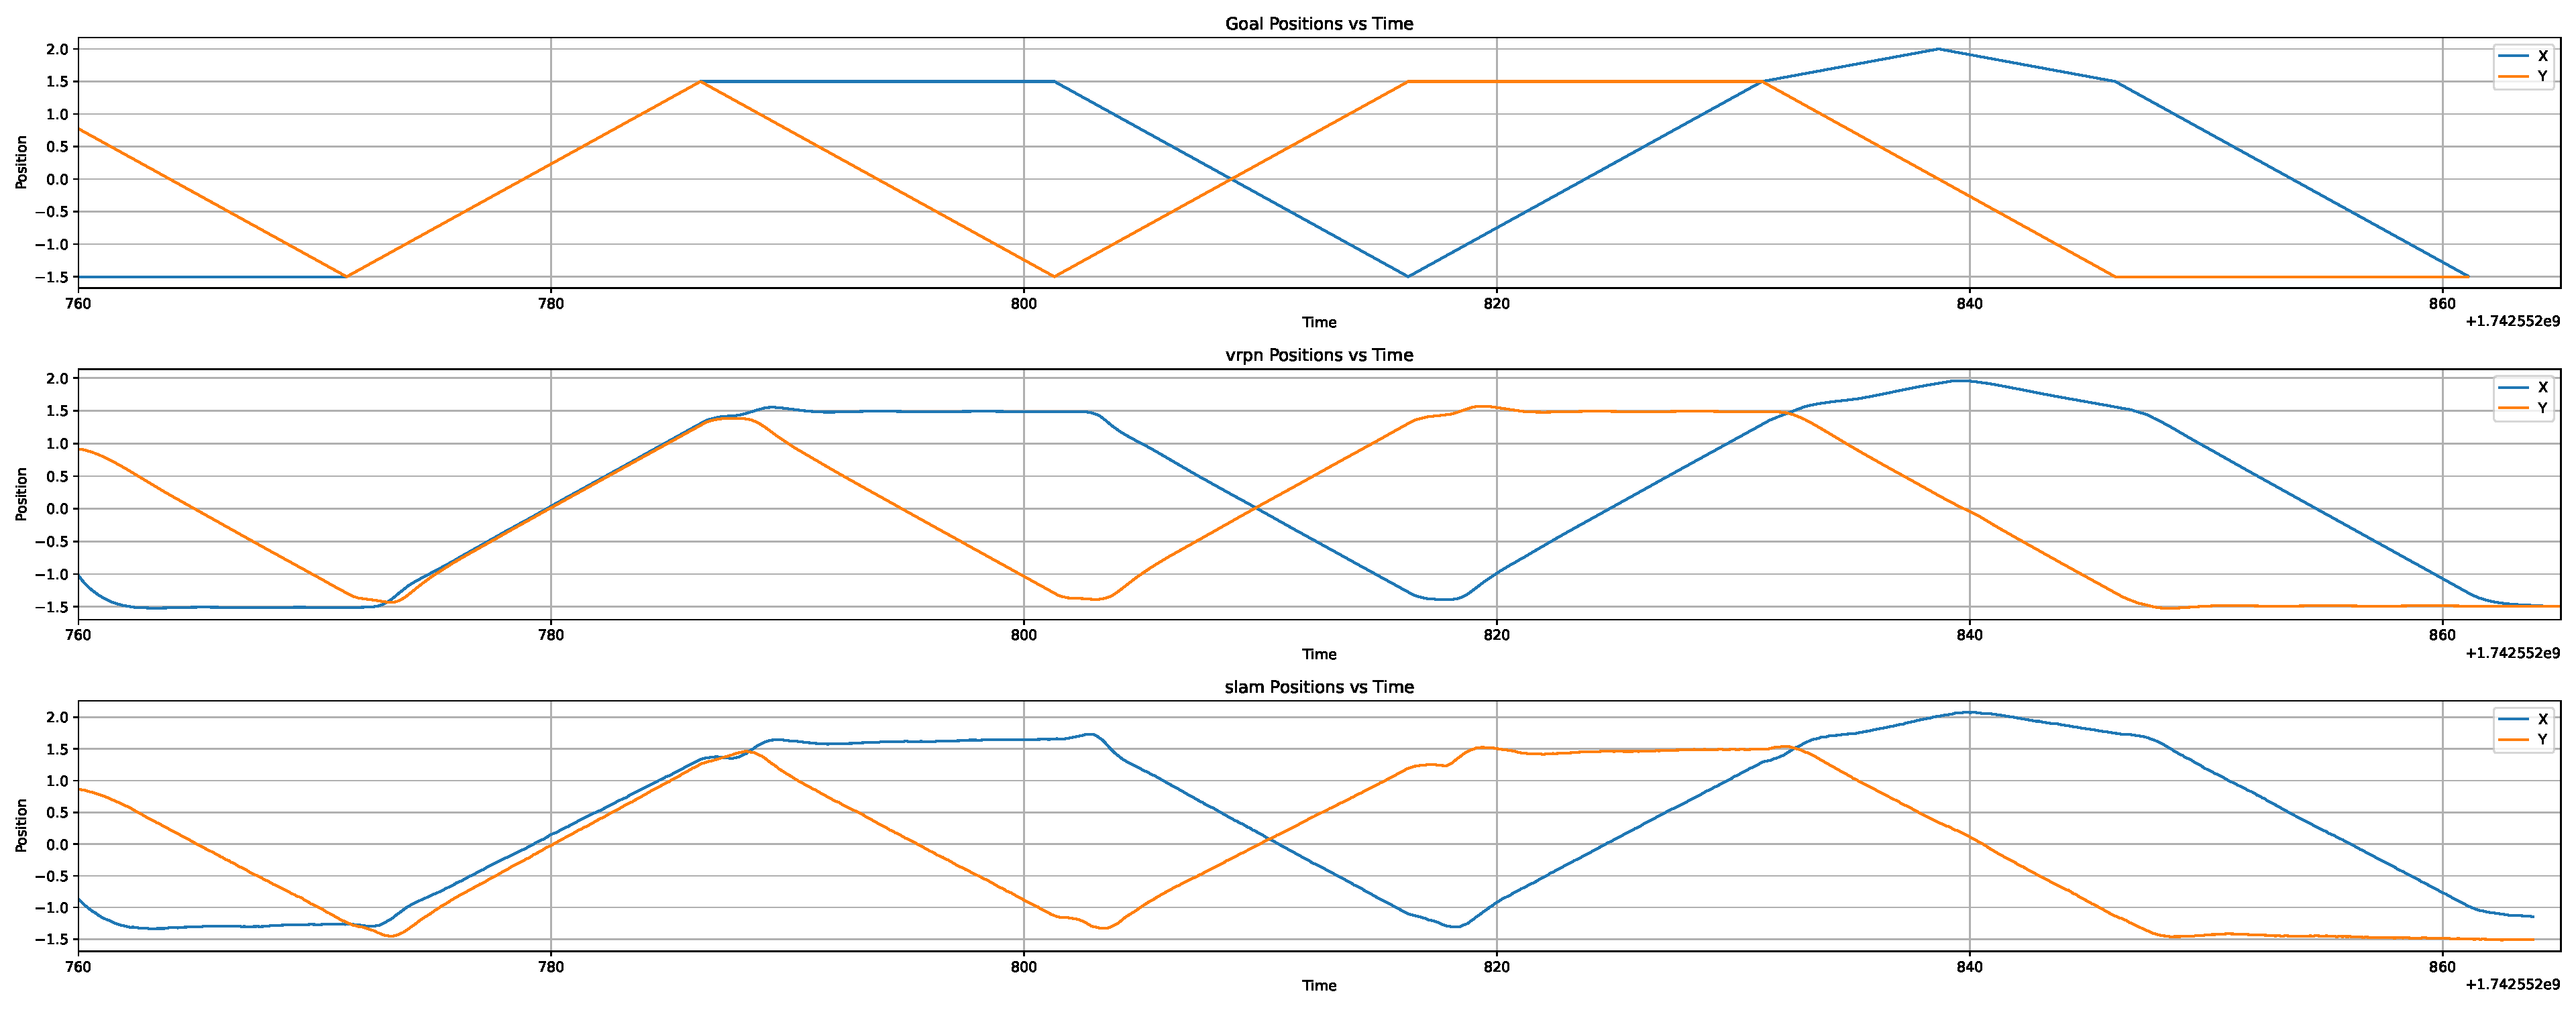
\includegraphics[width=1\linewidth]{img/Resultados/Exp1_VRPN_Control_LINEAR/Posicoes_v_tempo.pdf}
    \caption{Enter Caption}
    \label{fig:enter-label}
\end{figure}

\begin{figure}
    \centering
    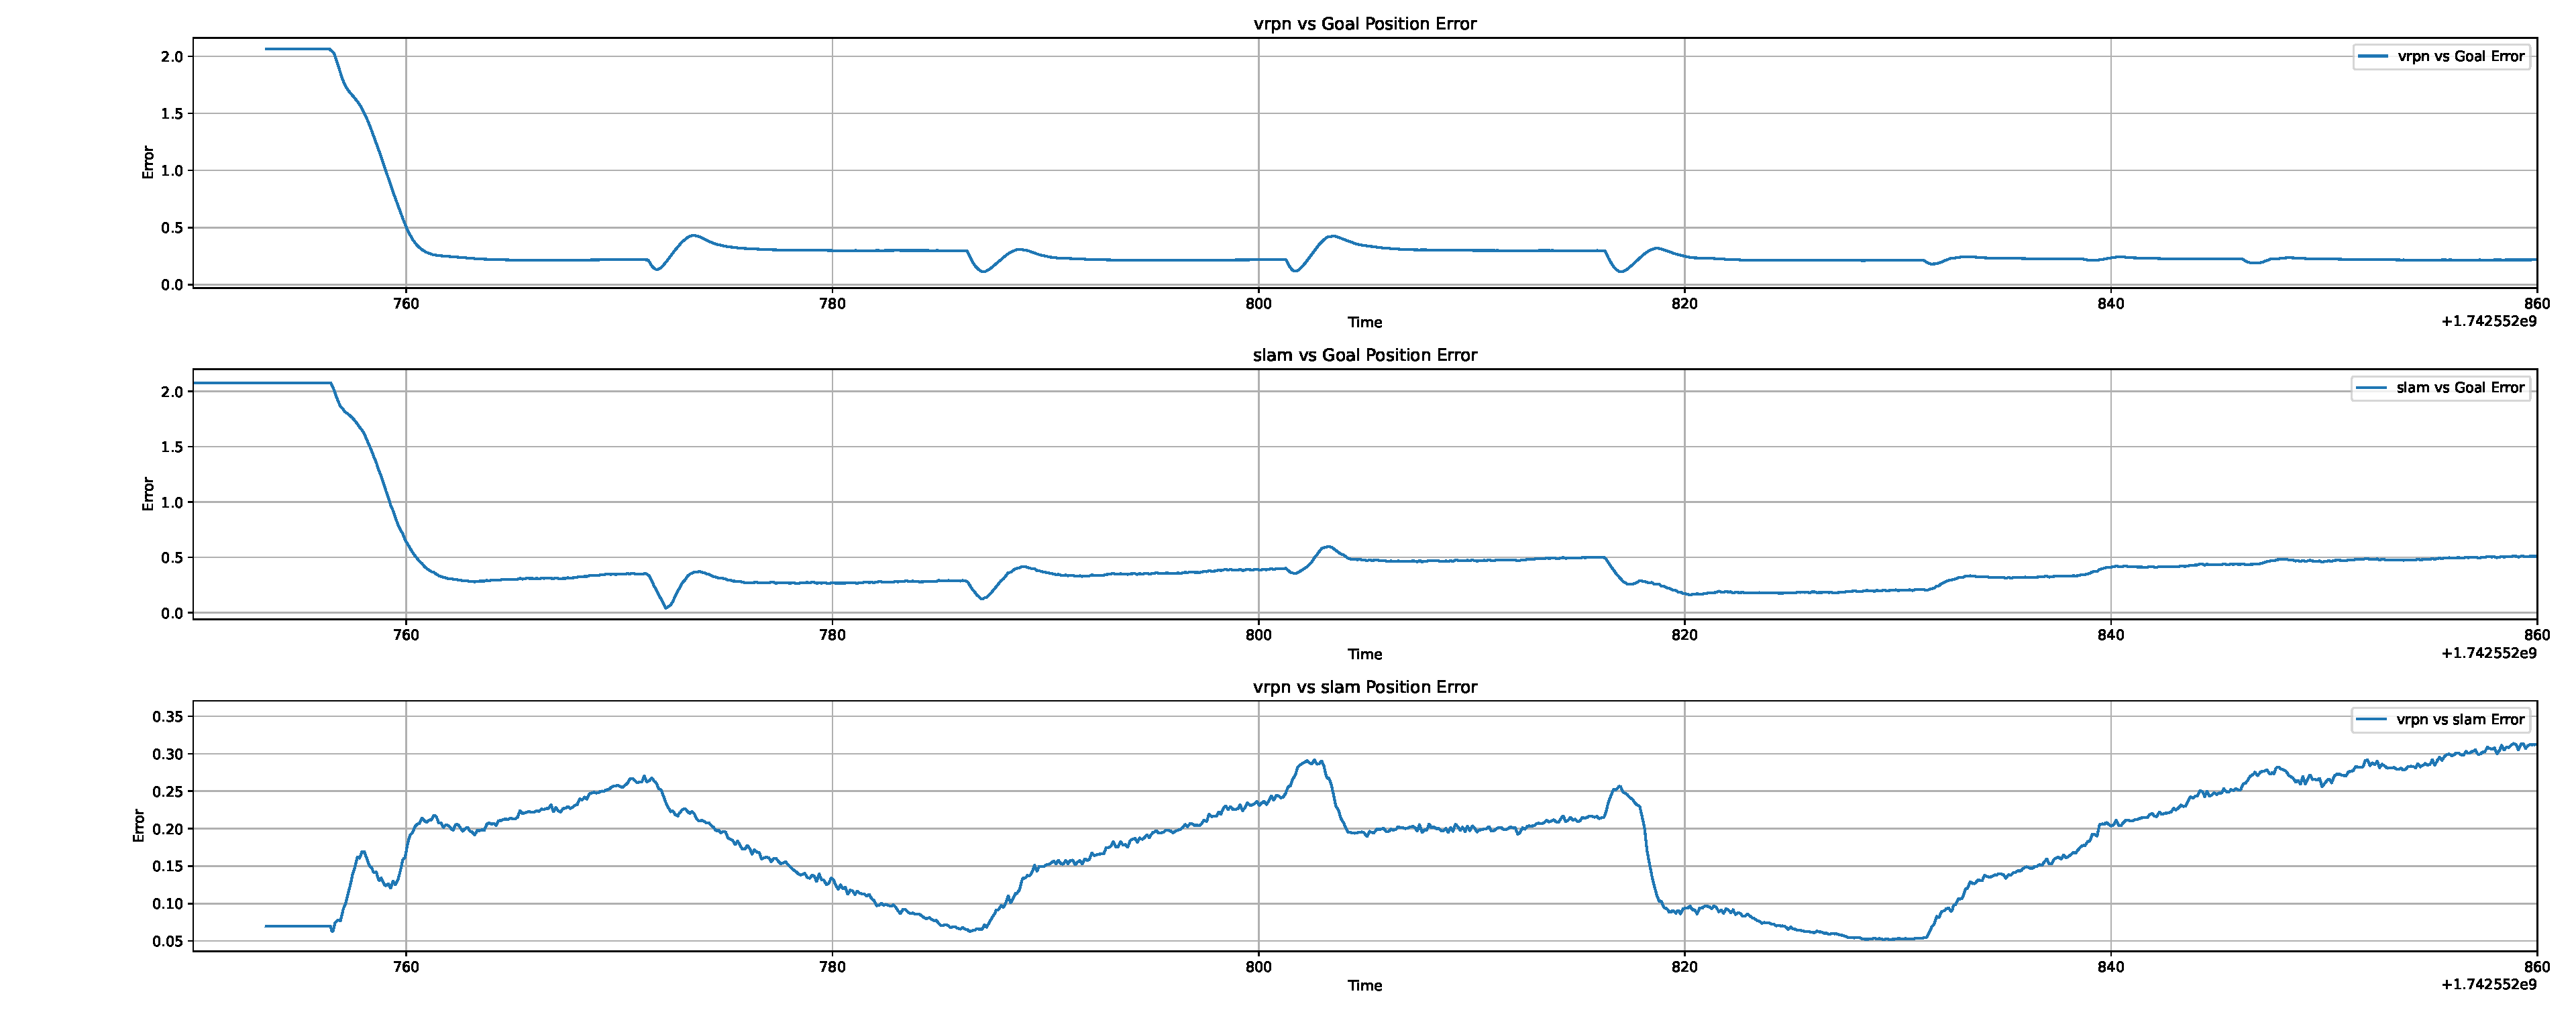
\includegraphics[width=1\linewidth]{img/Resultados/Exp1_VRPN_Control_LINEAR/Erros.pdf}
    \caption{Enter Caption}
    \label{fig:Exp1_Erros}
\end{figure}

A segunda trajetória realizada no segundo e quarto experimentos foi uma trajetória em formato de lemniscata de Bernoulli, caracterizada pelas equações:

\begin{equation}
    \bs{x}_{des}=\begin{bmatrix} x_{des}=r_x\cos{\omega t} \\ y_{des}=r_y\sin{2 \omega t} \end{bmatrix}
\end{equation}

com $r_x = 1.5m$, $r_y = 1.0m$ e $\omega = 0.20\ Rad/s$. A velocidade desejada da trajetória é obtida pela derivada da equação anterior:

\begin{equation}
    \dot{\bs{x}}_{des}=\begin{bmatrix} \dot{x}_{des} = -r_x \omega \sin{\omega t} \\
    \dot{y}_{des}=r_y 2\omega\cos{2 \omega t} \end{bmatrix}
\end{equation}

A Figura \ref{fig:Exp2_TrajetoriaVRPN} mostra o trajeto realizado pelo robô em comparação com a trajetória desejada no Experimento 2.

\begin{figure}
    \centering
    \caption{Experimento 2 - Trajetória desejada e realizada pelo robô}
    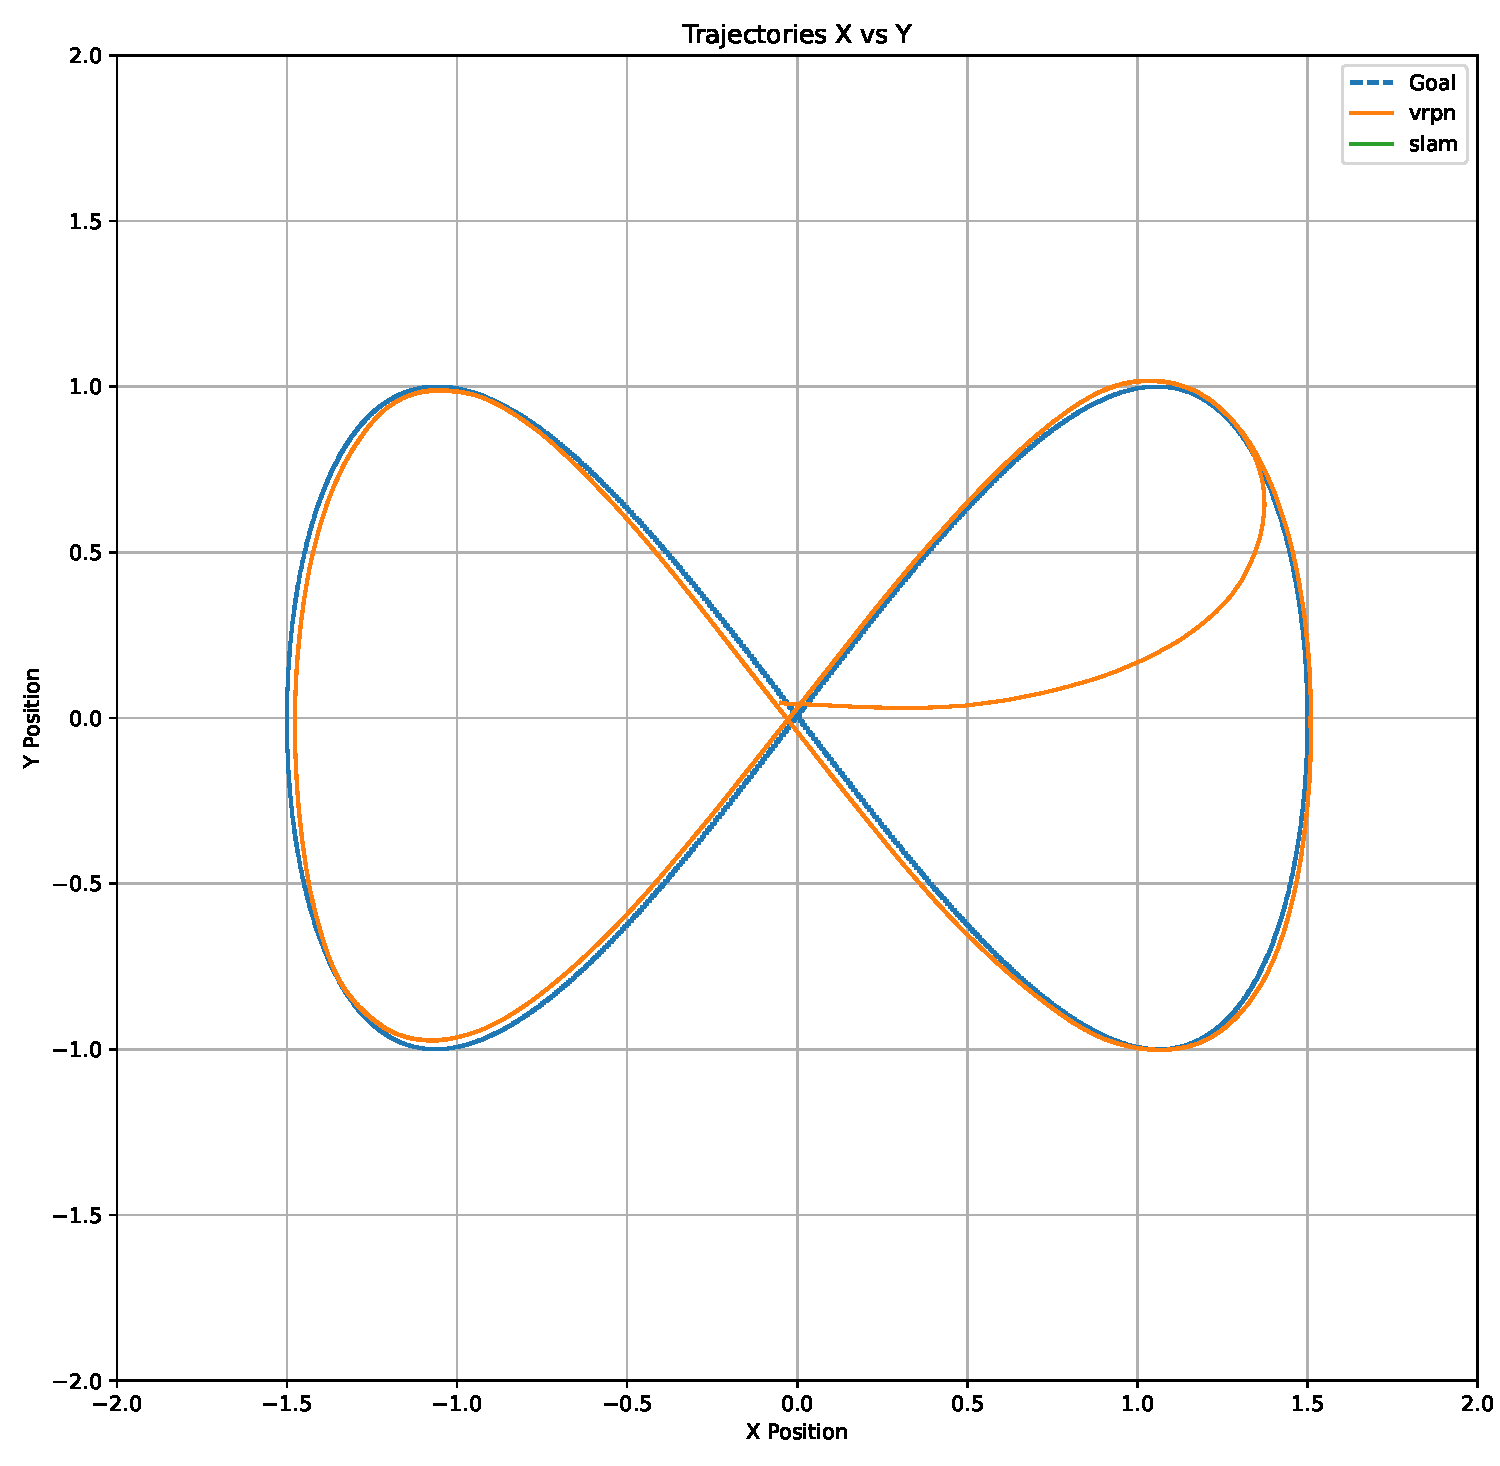
\includegraphics[width=0.8\linewidth]{img/Resultados/Exp2_VRPN_Control_LEMNISCATA/Trajetoria_VRPN.pdf}
    \source
    \label{fig:Exp2_TrajetoriaVRPN}
\end{figure}

% \begin{figure}
%     \centering
%     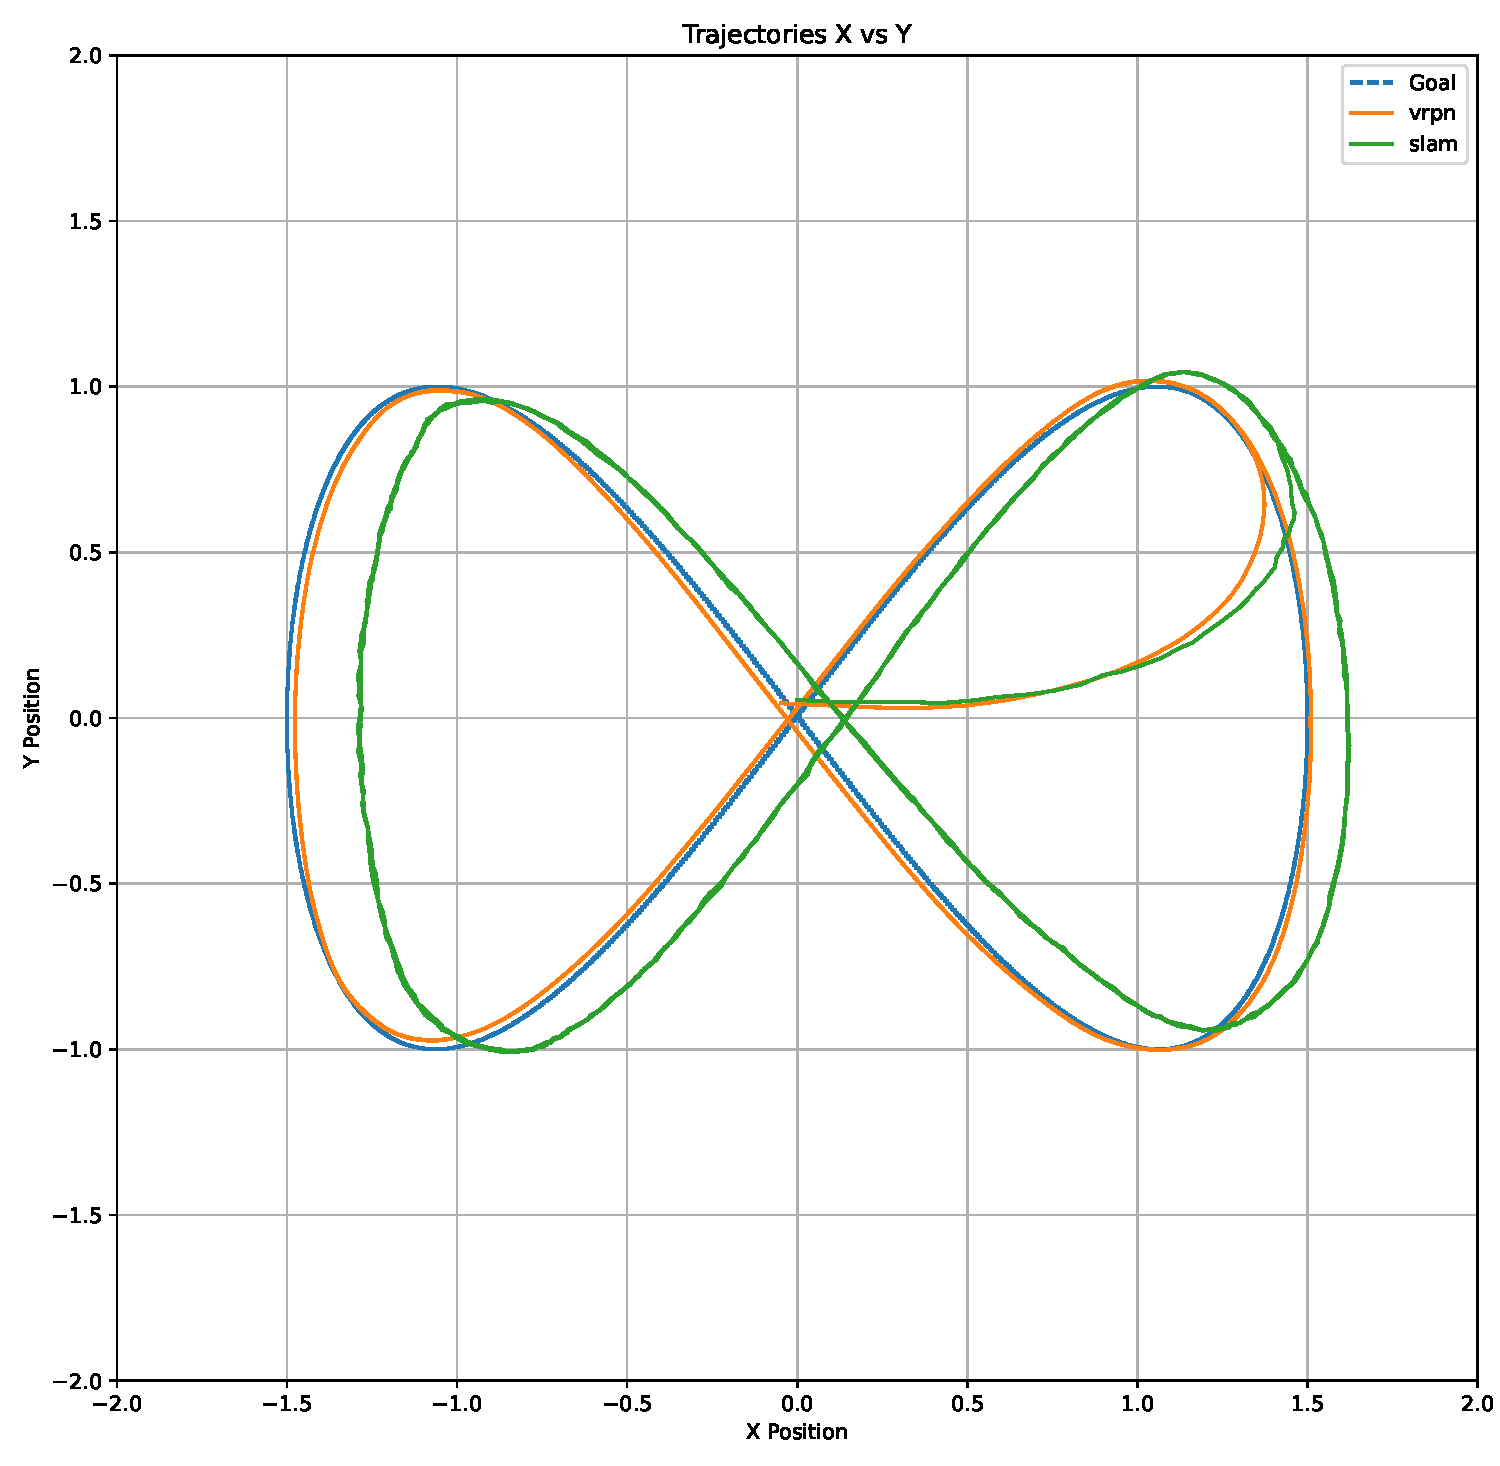
\includegraphics[width=\linewidth]{img/Resultados/Exp2_VRPN_Control_LEMNISCATA/Trajetoria_ALL.pdf}
%     \caption{Enter Caption}
%     \label{fig:Exp2_Trajetoria_All}
% \end{figure}

% \begin{figure}
%     \centering
%     \caption{Experimento 2 - Evolução das Posições no tempo do experimento}
%     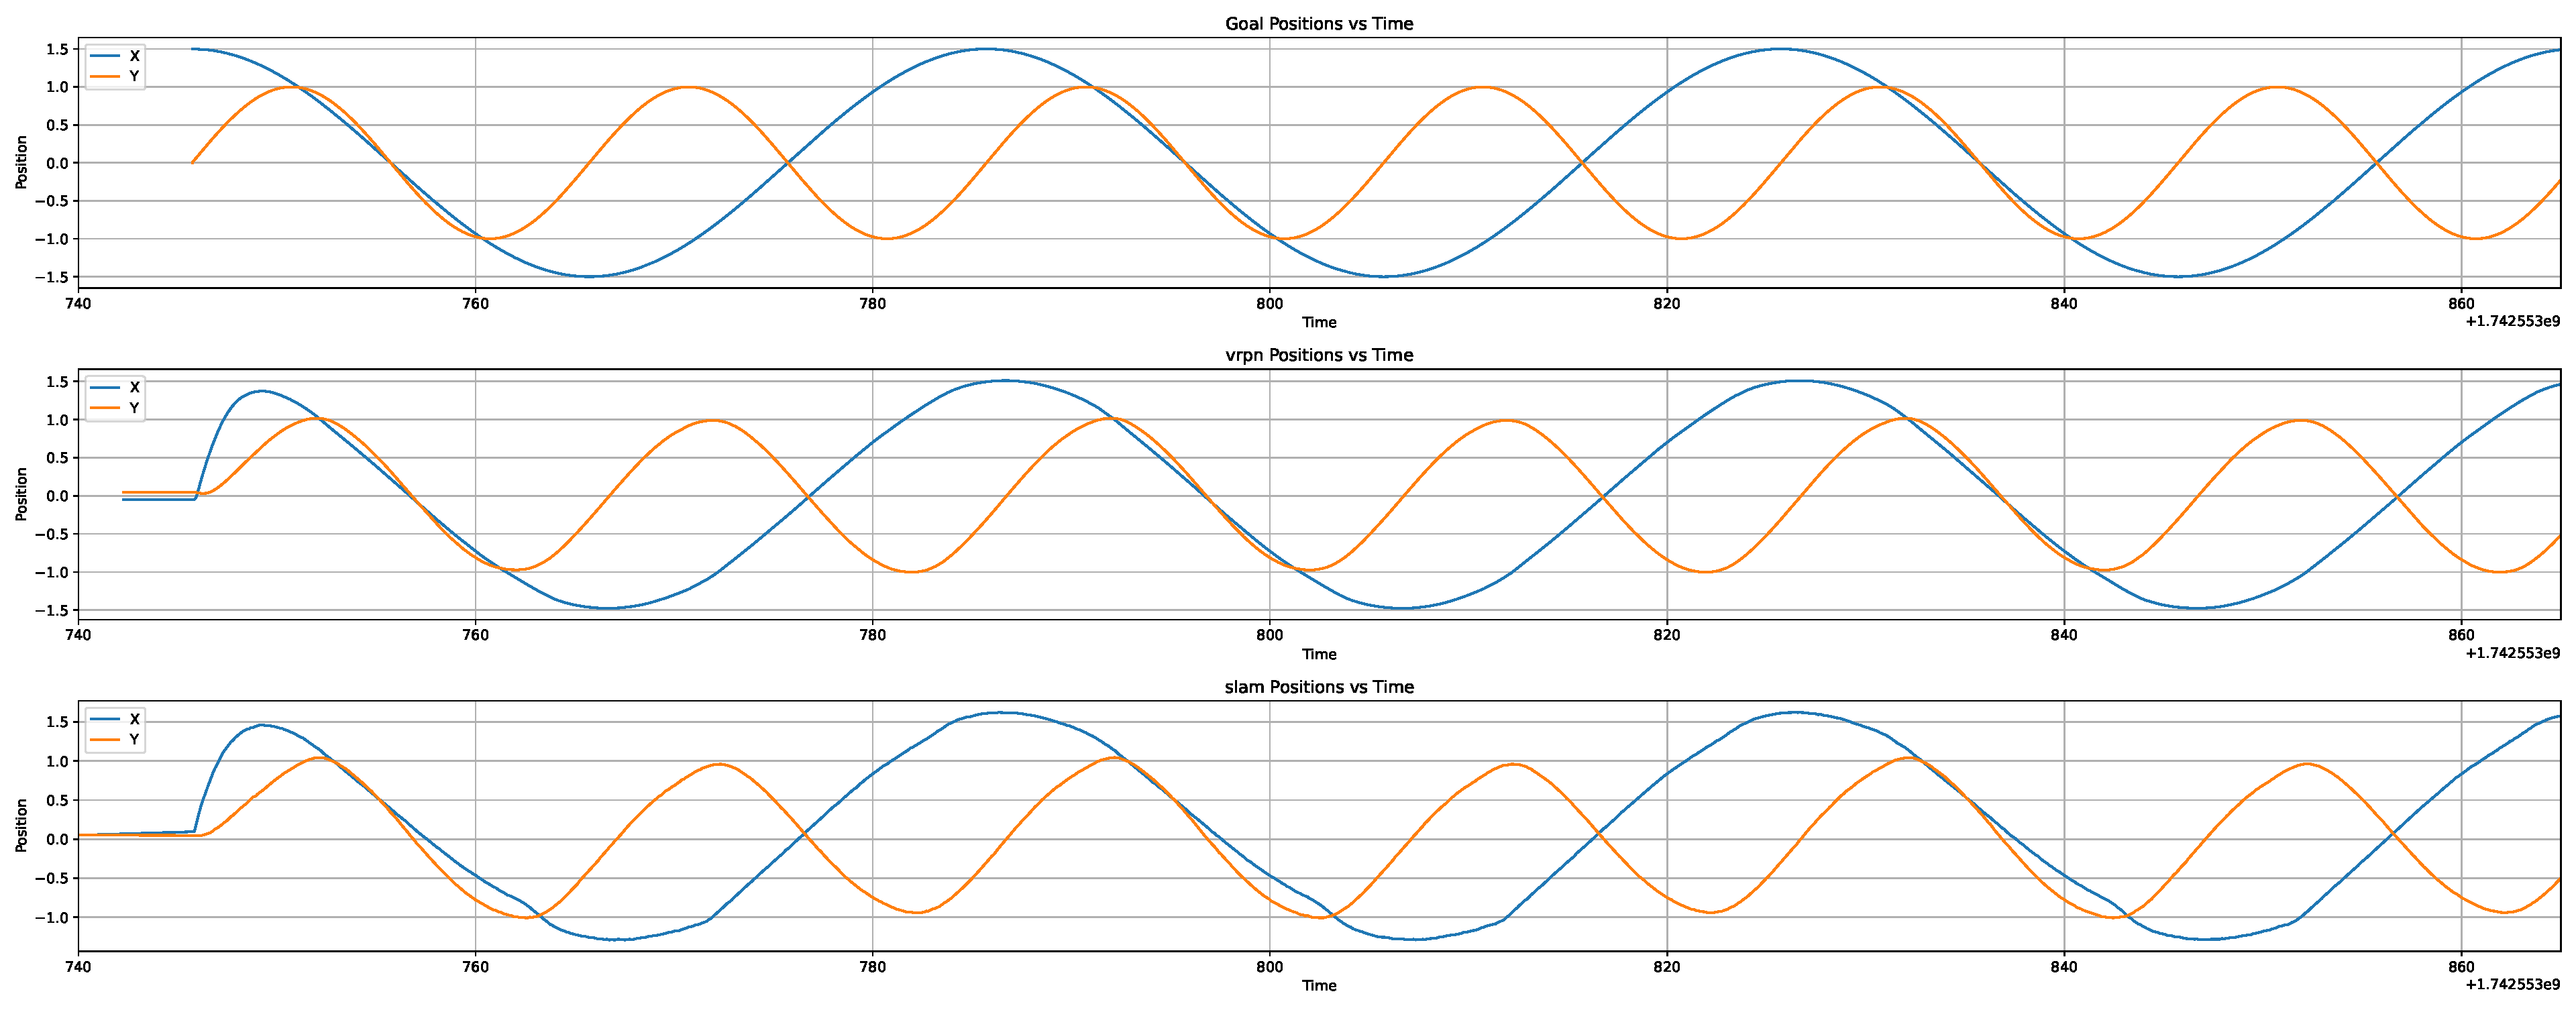
\includegraphics[width=\linewidth]{img/Resultados/Exp2_VRPN_Control_LEMNISCATA/Positions_v_Time.pdf}
%     \source
%     \label{fig:Exp2_PosicoesXY_v_tempo}
% \end{figure}

\begin{figure}
    \centering
    \caption{Experimento 2 - Comparação entre as posições registradas pelo OptiTrack e pela SLAM Toolbox durante o experimento}
    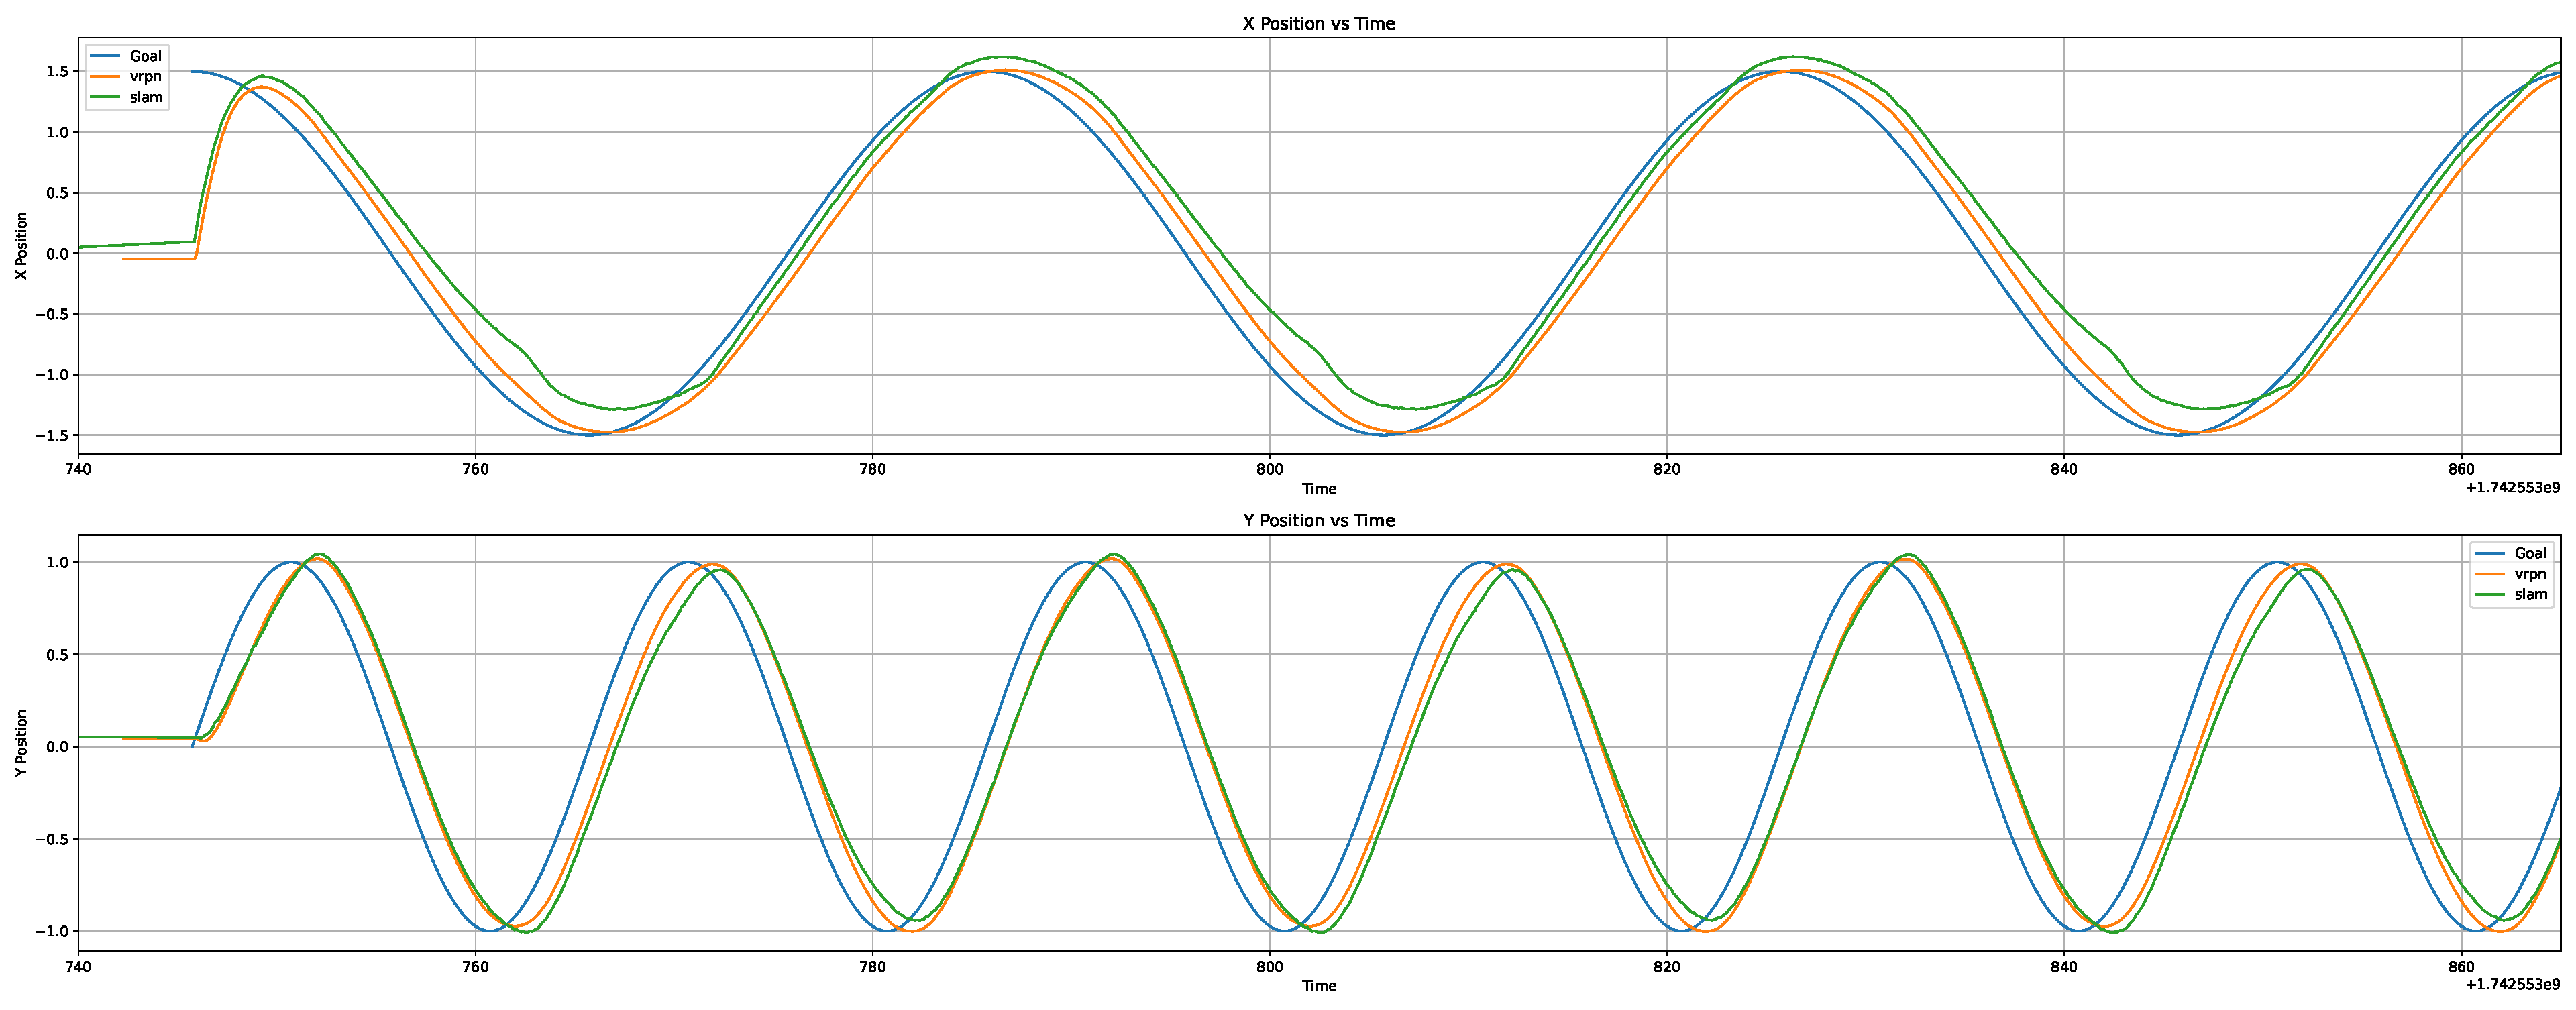
\includegraphics[width=\linewidth]{img/Resultados/Exp2_VRPN_Control_LEMNISCATA/PositionXY_v_Time.pdf}
    \source
    \label{fig:Exp2_Comparacao_Posicao_v_tempo}
\end{figure}

\begin{figure}
    \centering
    \caption{Experimento 2 - Erros de Posição}
    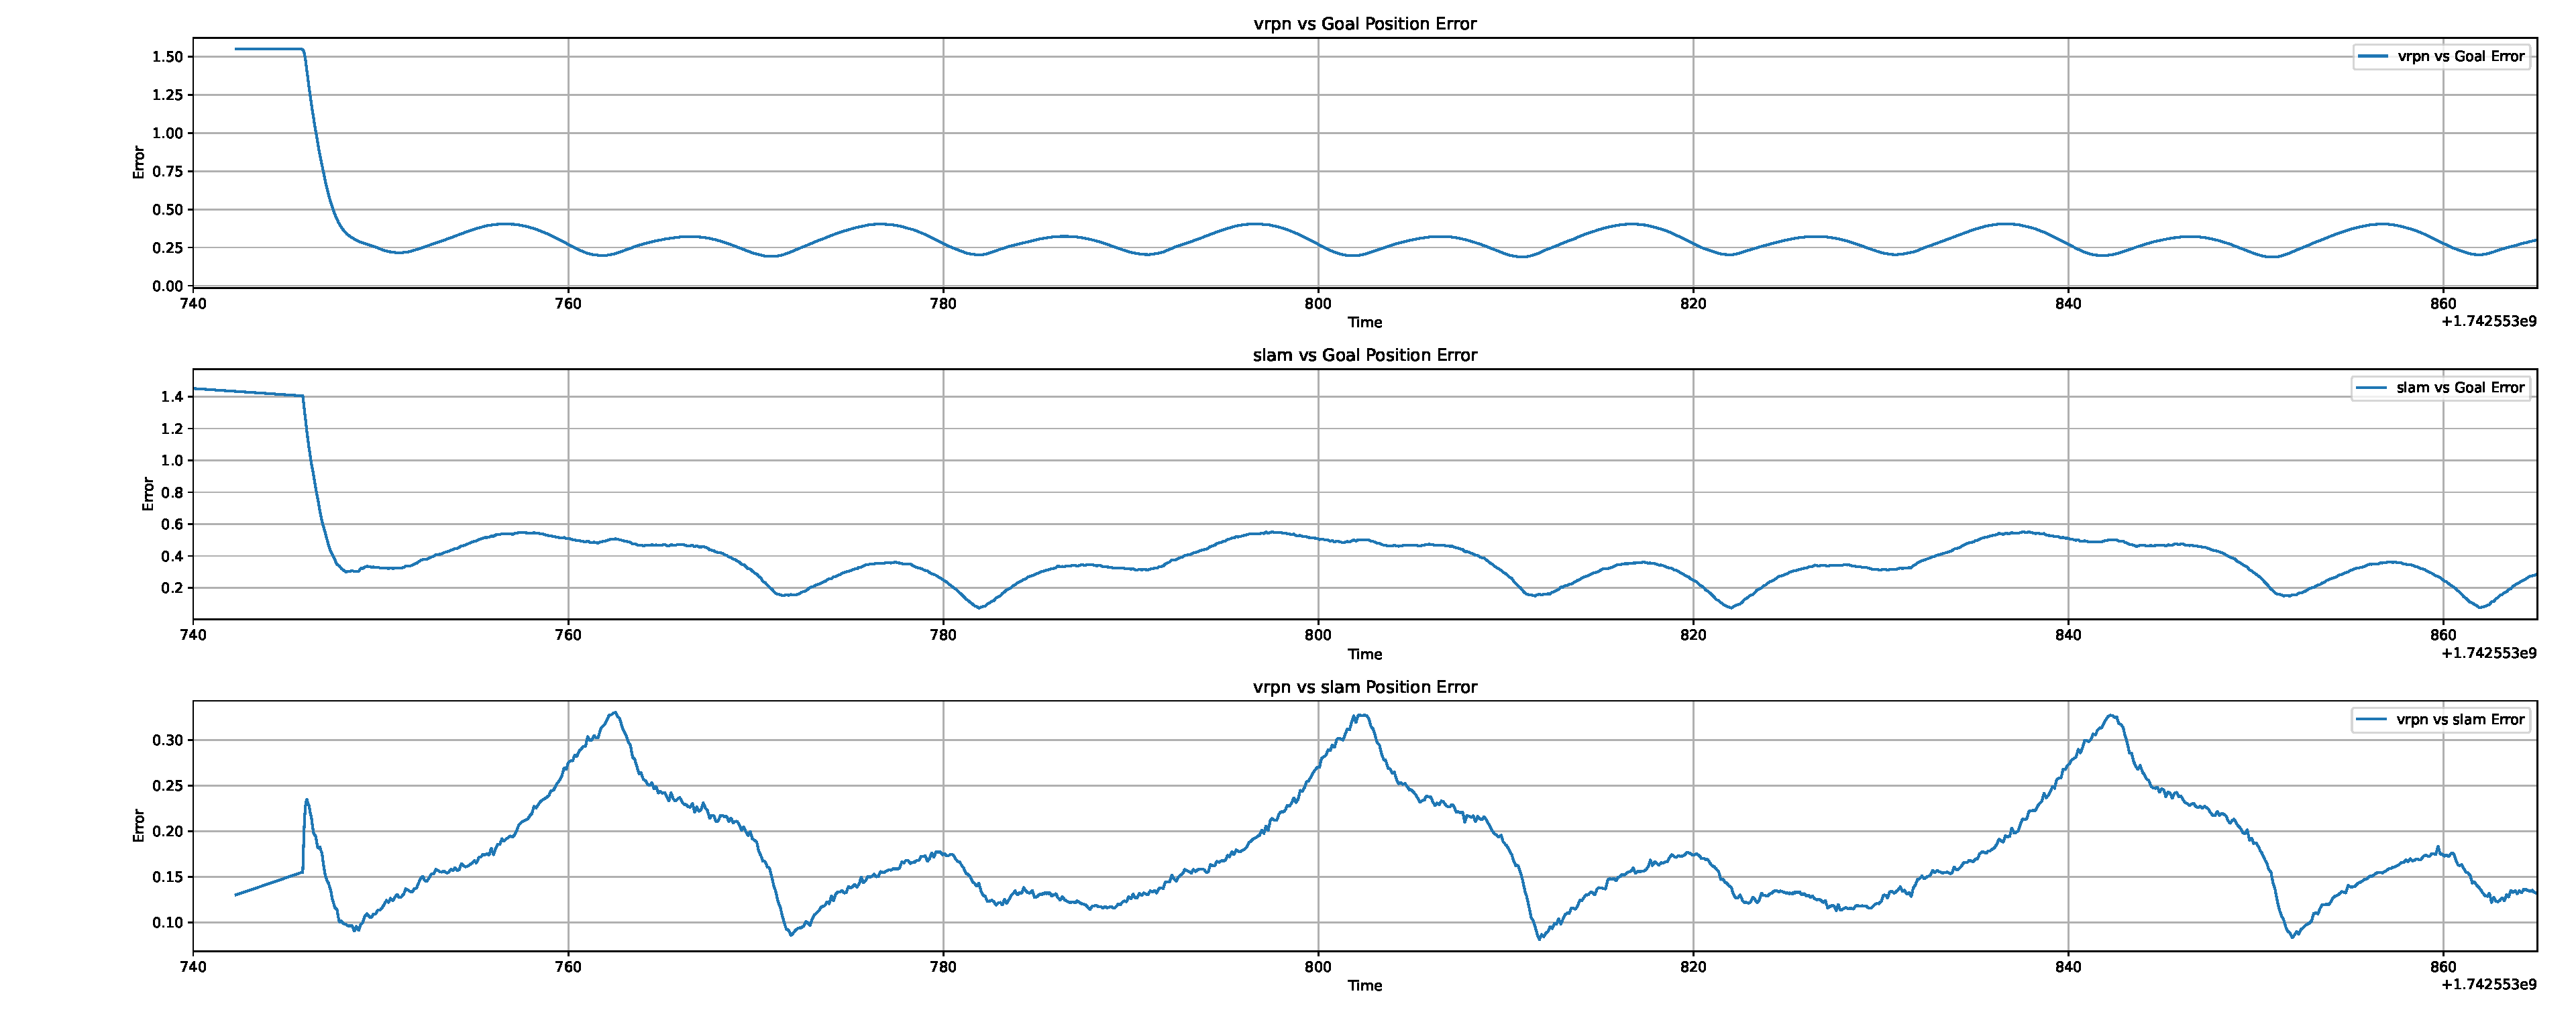
\includegraphics[width=\linewidth]{img/Resultados/Exp2_VRPN_Control_LEMNISCATA/Erros_Posicao.pdf}
    \label{fig:Exp2_Erros_Posicao}
\end{figure}